% ============================================================================
% 中文注释：第 6 节 实验（Experiments）
% ----------------------------------------------------------------------------
% 五小节：
%   6.1 主表：公开方法 + identity + 我们两臂。注意"我们比最好的公开方法高 +2.0 dB 是靠过平滑
%       换来的"（LapVar 比 0.60）——这一句必须写，否则等于自吹。
%   6.2 L_quiet：三种子 +0.50（CI [+0.34,+0.67]，14/15）；五种子 22.86±0.36；
%       **诚实点**：增益不集中在 Ω（22.30→22.39），所以不主张它修好遮挡区；
%       **不冗余**：去掉区域项只剩 19.53 / 20.26，说明两项互补。
%   6.3 哪一项吃重：区域项 4.16 > 梯度排斥 1.17 > 重建一致 1.12 > hinge 0.37；
%       L_r 原本是死的（分母 bug），按 RDNet 原版复活后单种子 +1.22、三种子 +0.18（噪声内）。
%   6.4 域消融：May 21.79 / Apr 20.72 / Jun(44) 20.57 / Jun(1093) 20.35 / 零样本 20.05。
%       关键解释：1093 对没用是**GT 错位**（88.7% >3px），对齐后 21.43；只筛掉最烂 99 对就 +0.80。
%   6.5 负结果表：两个结构方案是被 41–160 秒的 CPU 探针提前否掉的（省 12 GPU·h）；
%       权重平均 20.78 说明三种子落在不同 basin，种子方差不是噪声。
% 引用注意：所有 PSNR 来自同一冻结评测脚本（读 uint8 PNG），不是训练日志里的浮点值。
% ============================================================================
\section{Experiments}
\label{sec:experiments}

% 中文：统一配方（冻结 FocalNet、6000 it、bs4、30% 真实/40% 在线合成/30% 开源直督），
% 训练池来自 5 月+6 月共 174 对/7 场景；所有数字由同一个评测脚本产出。
\paragraph{Setup.}
Unless stated otherwise all arms use the same recipe: RDNet with a frozen FocalNet backbone,
$6000$ iterations, batch $4$, Adam at $10^{-4}$, random crops $224\!\rightarrow\!256\! \rightarrow\!320$,
$30\%$ real pairs / $40\%$ online-synthesised pairs / $30\%$ public SIRR pairs. Training pools are
built from a $5$-month and a $6$-month capture ($174$ pairs, $7$ scenes). Every number in
Tab.~\ref{tab:main} is produced by the same frozen evaluation script, which reads the stored
uint8 PNG predictions.

\subsection{Main results}

% 中文：两条读法——(a) 所有方法在 Ω 内都是负的，我们只是把伤害从 −3.4 减到 −2.2；
% (b) 我们 +2.0 dB 的领先是靠过平滑换的（LapVar 比 0.60），所以 PSNR 只当一个坐标看。
Tab.~\ref{tab:main}. Two observations.
\emph{(a)} All public methods are more than $3\dBA$ worse than identity inside $\Om$, and the
fine-tuned models reduce that damage to $-2.2\dBA$ without ever becoming safe: the occluder region
remains the region where SIRR hurts, for every method we tested.
\emph{(b)} The aggregate gap between our baseline and the best public method ($+2.0\dBA$) is
obtained at the cost of over-smoothing: the LapVar ratio is $0.60$ for our model (identity $1.0$),
while HF-PSNR and gradient cosine are comparable. We therefore treat PSNR as one coordinate of the
result, not as the result.

\subsection{The change-aware regularizer}
\label{sec:exp:quiet}

% 中文：逐场景 Δ 图——14/15 为正，均值 +0.50，CI [+0.33,+0.67]；唯一为负的场景只有 −0.07（噪声内）。
\begin{figure}[t]
\centering
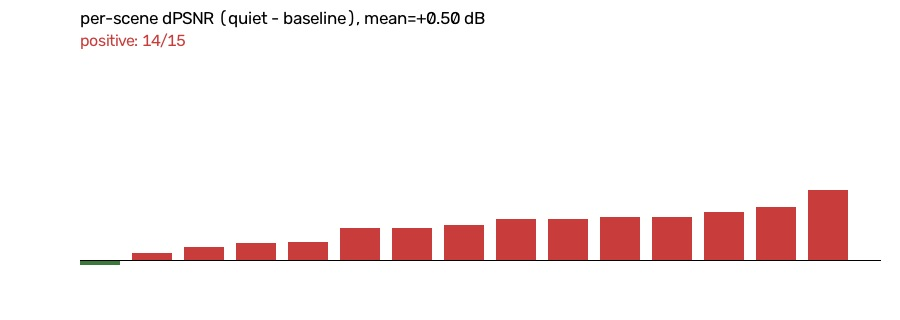
\includegraphics[width=\linewidth]{fig/perscene.jpg}
\caption{\textbf{Per-scene effect of $\quiet$} (mean of three seeds, minus the three-seed
baseline). Bars sorted by gain; $14$ of $15$ scenes improve, mean $+0.50\dBA$, $95\%$ CI
$[+0.33,+0.67]$. The single loss is $-0.07\dBA$, i.e.\ within measurement noise.}
\label{fig:perscene}
\end{figure}

% 中文：三种子 22.99±0.34 vs 基线 22.49±0.44；五种子 22.86±0.36。
% **必须写明种子轴 CI 仍跨 0**——我们只能主张逐场景稳健，不能主张跨种子稳健。
\paragraph{Seeds.} $\quiet$ ($\lambda=1$, $\tau=0.05$) gives $22.99\pm0.34$ over three seeds
($22.71/23.38/22.88$) versus $22.49\pm0.44$ for the baseline ($21.99/22.84/22.62$). The paired
per-scene improvement is $+0.50\dBA$ with a $95\%$ CI of $[+0.34,+0.67]$ and is positive on
$14/15$ scenes; a five-seed run gives $22.86\pm0.36$. The \emph{seed-level} interval, however, still
contains zero ($[-0.07,+1.08]$): with three seeds we can claim per-scene robustness but not
seed-level robustness, and we report it as such.

% 中文：λ=5 反而略低（+0.44）但 15/15 全正、种子方差最小 ⇒ 它更像"约束"而非"新目标"。
\paragraph{Strength.} $\lambda=5$ gives $+0.44\dBA$ with $15/15$ scenes positive and the smallest
seed spread ($22.92\pm0.16$). Increasing $\lambda$ does not give more, which is consistent with the
regularizer acting as a \emph{constraint} rather than as an additional objective.

% 中文：诚实点——收益**不**集中在 Ω（22.30→22.39，仅 +0.09），所以不主张它解决遮挡区问题；
% 它阻止的是"在不该动的地方动"，效果摊在全图上。
\paragraph{It is not a region fix.} The gain is \emph{not} concentrated inside $\Om$
($22.30\rightarrow22.39\dBA$, i.e.\ $+0.09$), so we explicitly do not claim that $\quiet$ solves
the occluder problem of Sec.~\ref{sec:axis1}. What it does is prevent the model from moving pixels
that need no change; the benefit is spread over the whole frame, and the fourteen scenes that gain
do so on non-$\Om$ content.

% 中文：但也不冗余——把区域项关掉只留 L_quiet，只有 19.53（连 hinge 也关掉是 20.26），
% 远低于两者同时用的 22.99。⇒ 区域项供大头，L_quiet 追加增量。
\paragraph{It is not redundant with the masked term.} Removing the annotation entirely and keeping
only $\quiet$ is much worse than keeping both: with $\lambda_\Om=0$ and $\quiet$ active the panel
score is $19.53\dBA$ (and $20.26\dBA$ if the hinge term is also disabled), against $18.33\dBA$ for
$\lambda_\Om=0$ alone and $22.99\dBA$ for the full model. The two terms are therefore
\emph{complementary}: Eq.~\eqref{eq:lom} supplies the bulk, $\quiet$ adds the rest.

\subsection{Which loss terms are load-bearing}

% 中文：留一法（单种子、同池）。区域项 4.16 最大；梯度排斥 1.17；重建一致 1.12；hinge 0.37；
% L_r 原本数值上是死的（分母多乘 hw），按 RDNet 原版复活后单种子 +1.22 但三种子只有 +0.18（噪声内）。
We remove one term at a time from the nine-term objective (single seed, same pool). Removing the
reconstruction consistency $|I-\That-\Rhat|$ costs $1.12\dBA$; removing the gradient-exclusion term
costs $1.17\dBA$; removing the overshoot hinge costs $0.37\dBA$; the region term costs
$4.16\dBA$ (Sec.~\ref{sec:axis3}). The reflection-column term contributes $+0.02\dBA$---we later
found it had been numerically dead (a normalisation bug) and that reviving it in RDNet's original
squared form yields $+1.22\dBA$ on one seed but only $+0.18\dBA$ over three ($23.21/22.51/22.27$),
i.e.\ inside the seed spread. DISTS and the Laplacian fidelity term contribute $+0.08$ and
$+0.07\dBA$. This ordering is stable across pools.

\subsection{Domain ablation: what makes a real pair useful?}

% 中文：同配方换域：May 21.79 / Apr 20.72 / Jun(2 场景,44 对) 20.57 / Jun(13 场景,1093 对) 20.35，
% 零样本 20.05 ⇒ **1093 对等于白给**，与样本量直觉相反。
\paragraph{Domain ablation.}
Training the same recipe on different capture months, one domain at a time, gives
$21.79$ (May), $20.72$ (April), $20.57$ (June, $2$ scenes) and $20.35$ (June, $1093$ pairs,
$13$ scenes) against $20.05$ for the zero-shot model. A $1093$-pair pool is thus worth
\emph{nothing}, which is the opposite of what its size suggests.

% 中文：原因不是域漂移，是**几何错位**：88.7% 的对位移 >3px（中位 8.2px），因为 T 是手持片段最后一帧。
% 对齐后 21.43；只丢掉最烂的 99 对就已从 20.35 升到 21.15。⇒ GT 对齐是 SIRR 训练数据的一阶属性。
The cause is not domain shift:
phase correlation shows that $88.7\%$ of those pairs have $T$ misaligned with $I$ by more than
$3$\,px (median $8.2$\,px), because $T$ is the last frame of a handheld clip. After per-pair
translation alignment the same pool reaches $21.43\dBA$ (single seed), and merely \emph{discarding
the worst $99$ pairs} already improves the unaligned pool from $20.35$ to $21.15\dBA$. Ground-truth
alignment is therefore a first-order property of SIRR training data, and we recommend reporting the
alignment distribution alongside the pair count.

% 中文：混训的结果——Ω 抬上去了，但 β 掉下来，说明是"少动"不是"学会补图"。
\paragraph{Mixing occluder-rich data improves $\Om$ but not the task.}
Since the occluder region is where models fail, one may try to fix it with data. Mixing
our $11$-month indoor capture into the $5{+}6$-month pool raises $\mathrm{PSNR}_\Om$ from
$20.91$ to $23.76\dBA$ at a $50{:}50$ ratio, and the gain is broad---positive on
$15/15$ scenes, mean $+2.84\dBA$. It is also misleading: the same arm moves from $\beta=-0.34$
to $-0.47$ and its action ratio (mean $|\That-I|$ over mean $|I-T|$) drops from $0.79$ to
$0.60$, i.e.\ it wins $\Om$ by \emph{doing less}. At $75\%$ the pool reaches
$\mathrm{PSNR}_\Om=23.78$ with $\beta=-0.63$ and an action ratio of $0.43$. No mixture
beats the best single-domain model on the full metric ($22.38$ vs.\ $22.71$), so we read
this as further evidence that $\mathrm{PSNR}_\Om$ alone does not identify progress.

\subsection{Negative results}
\label{sec:negative}

% ============================================================================
% 中文注释：表 2 负结果（单栏）
% ----------------------------------------------------------------------------
% 三组，用横线隔开：
%   ① 针对 Ω 内容恢复的尝试（全部失败，且**都能从 §4.3 的"同频段"解释**）
%       感知损失（LPIPS/GAN 式）—— 对冲求稳：mean-seeking，多解时取平均
%       把输入高频拼回 Ω —— 结构回到 1.31×，但 PSNR 掉 0.22–0.31 dB（把反射也搬回来了）
%       加遮挡区数据混训 —— Ω 抬 +2.84 dB（15/15），但 β 从 −0.34 退化到 −0.47、
%                              动作比 0.79→0.60：是"少动"不是"学会补图"
%   ② 真的训练过的其它臂
%   ③ 被 CPU 探针提前否掉的（省 GPU 时）
% 注意：这张表不是"实验失败记录"，而是"哪条路已被证否"的证据；不要因为都是负的而删。
% ============================================================================
\begin{table}[t]
\centering
\caption{Negative results. ``Probe'' rows were rejected by a CPU-only learnability probe
before any training run. The first block are attempts to \emph{recover the content of
$\Om$}; all fail, and Sec.~\ref{sec:band} explains why.}
\label{tab:negative}
\footnotesize
\setlength{\tabcolsep}{3pt}
\begin{tabular}{@{}p{0.48\linewidth}p{0.46\linewidth}@{}}
\toprule
Proposal & Result / verdict \\
\midrule
perceptual loss inside $\Om$ & hedged / averaged, no gain \\
splice input $\mathrm{HF}$ into $\Om$ & $-$0.22 (struct.\ $1.31\times$) \\
mix $25$--$50\%$ occluder data & $\Om$ $+2.84$ but $\beta$ $-0.34\!\to\!-0.47$ \\
extra synthetic pairs & $22.34$ vs $22.38$, null \\
\midrule
$8{\times}8$ photometric adapter ($+18$k) & $-0.06$, fail (3 seeds) \\
input-side rescaling to match $g$ & $+0.19$, null (1 seed) \\
reweight gradient fidelity & $-0.18$, \emph{worse} \\
region-agnostic loss shift & $-0.34$, useful (kept) \\
deeper $L_1$ on reflection column & $+0.34$, below gate \\
final iterations with MSE & $+0.28$, below gate \\
\midrule
dual-dict.\ proximal separation & probe $-0.08$..$-0.26$, rejected \\
residual-magnitude gate ($1025$ par.) & probe $-0.29$, rejected \\
weight averaging of 3 seeds & $20.78$, fails (basins) \\
\bottomrule
\end{tabular}
\end{table}


% 中文：两点——① 三个结构方案都是被 41–160 秒的 CPU 探针提前否掉的（各省 6 GPU·h），
% 在效应量只有 ~0.3 dB、种子方差 0.44 的情况下，这种探针应当成为强制流程；
% ② 三种子权重平均 20.78 < 任一成员，说明种子落在不同 basin，观测到的方差不是"同一解附近的噪声"。
Tab.~\ref{tab:negative} lists proposals that did not work. Two comments. First, the
\emph{structural} proposals (a photometric adapter of $18$k parameters, a residual-magnitude gate
of $1025$ parameters, a dual-dictionary proximal layer separation) were all falsified by a
\emph{CPU-only probe}: fit the candidate's last layer on training scenes and evaluate on held-out
scenes. The probes take $41$--$160$ seconds and each saved a $6$ GPU-hour training run. Given that
the effect sizes we can resolve are $O(0.3\dBA)$ and the seed spread is $0.44\dBA$, we consider such
probes mandatory rather than optional. Second, weight averaging of three seeds fails catastrophically
($20.78\dBA$, i.e.\ below any of its constituents): the seeds sit in different basins, so the
per-scene variance we observe is \emph{not} noise around a common solution.
